\documentclass[12pt,a4paper,oneside]{report}
% nagyon sok kép esetén meggyorsítható a fordítás a draft móddal
% \documentclass[12pt,a4paper,oneside,draft]{report}
% ekkor a képek nem renderelődnek ki, csak placeholder lesz mérethelyesen
\usepackage[magyar]{babel}
\usepackage[T1]{fontenc}
\usepackage{amsmath} 
\usepackage{amsfonts}
\usepackage{amssymb}
%\usepackage[sorting=none]{biblatex} [style=ieee] % <- emiatt megakad (nem akad meg amúgy), [sorting=none]: előfurdulás sorrendjébe rakja a hivatkozásokat
\usepackage{caption}
%\usepackage[hang]{caption}
\usepackage{enumerate}
\usepackage{epsfig} % eps importáláshoz
\usepackage{float} % képek pontos elhelyezéséhez: \begin{figure}[H]
\usepackage{graphics} % grafikus elemek, képek berakásához
\usepackage{graphicx}
\usepackage{hyperref} % PDF hivatkozásokhoz kell
\usepackage{hyphenat} % elválasztáshoz
\usepackage{url}
\usepackage[utf8]{inputenc} % mindenképp maradjon az utf-8 kódolás
\usepackage{lastpage}
\usepackage{listings}
\usepackage{mathcmd} % \Grad \Div \Rot \mathrm{dv}
\usepackage{sectsty}
\usepackage{setspace}
\usepackage{siunitx} % \SI{}{} \si{}
\usepackage{subcaption} % subcaption-hoz, pl: 3.2.2
\usepackage{titling} % a title, author parancsok szabad használatához
\usepackage{psfrag} % eps kép szövegéhez

% a TikZ rajzoló modul, és a kapcsolási rajz készítő modul, ha kell
%\usepackage{tikz}
%\usepackage{circuitikz}

% az A4 oldal margóinak és méreteinek beállítása
\usepackage[left=25mm,right=25mm,top=20mm,bottom=25mm]{geometry}\pagestyle{plain}

% A sorköz távolság beállítása
% egyszeres sorköz
\singlespacing
% 1,5 sorköz
% \onehalfspacing

% A hivatkozások, és linkek átállítása alapértelmezett színre, fekete-fehér nyomtatáshoz optimalizálva
\hypersetup
{
  	colorlinks,
  	citecolor=black,
 	linkcolor=black,
  	urlcolor=black
}


% a dolgozat címe
\newcommand{\dokumentumcim}{7. mérés: Szuperheterodin elvű rádió adó és vevő lánc mérése elv}

% a dolgozat típusa
\title{Rádióátviteli mérések laboratórium 2 (BMEVIHVMB02),\\
jegyzőkönyv beszámoló}

% konzulens
%\newcommand{\konzulens}{Konzulens: nincs} 

% a dolgozat szerzője
\author{HVT A csoport:\\
Horváth Péter (GV1A6F)\\
Kepics János (M74KL4)\\
Pintér Bálint (I6QS0K)\\
Szilágyi Gábor (NOMK01)}

% a dolgozat típusa - ez nincs a címlapon
\newcommand{\dokumentumtipus}{Szuperheterodin labor jkv}


% irodalomjegyzék forrása
%\addbibresource{szakdoga_irodalom.bib}

\begin{document}

\begin{titlepage}

\begin{figure}
	\centering
	
\includegraphics[width=100mm,keepaspectratio]{kepek/bme.pdf}
\end{figure}
%[scale = 1,bb=0 0 1280 960]
%
\centering
\textbf{Budapesti Műszaki és Gazdaságtudományi Egyetem}\\
\textbf{Villamosmérnöki és Informatikai Kar}\\
\textbf{Szélessávú Hírközlés és Villamosságtan Tanszék}\\
\vspace{5mm}

\includegraphics[width=40mm,keepaspectratio]{kepek/hvt_logo_only_fixed_vector_inverted.png}  \\

\vspace{40mm}
\Huge
\dokumentumcim\\
\vspace{6mm}%12mm

\Large
\thetitle \\
\vspace{6mm}

\Large
\textbf{\theauthor}\\ % név
%\vspace{40mm}
\vspace{30mm}

%\raggedright
%\konzulens\\ % konzulensek

%\vspace{6mm}

\centering
\the\year %dátum


\end{titlepage}
%\tableofcontents
%\include{bevezeto}
\section*{Áttekintés}

A mérés során vizsgált szuperheterodin elvű adólánc blokkvázlata a \ref{fig:ado}. ábrán látható. Az alapsávi jelet egy BPSK, illetve OOK modulációra képes modulátorral állítjuk elő, amit egy $\SI{16}{MHz}$-es vivőre kerül. Ezt szűrés után egy gyűrűs DBM keverő segítségével középfrekvenciára, $\SI{434}{MHz}$-re keverjük fel, a keveréshez $\SI{450}{MHz}$-es lokál oszcillátort (LO) használunk. KF szinten szűrés után felkeverjük a jelet $\SI{2.4}{GHz}$-es RF sávra egy PLL-es keverő segítségével. KF és RF fokozaton opcionálisan erősítőt is hozzáadhatunk az adólánchoz, ettől a mérés során eltekintettünk.

\begin{figure}[H]
	\centering
	\includegraphics[width=0.7\textwidth,keepaspectratio]{kepek/ado.PNG}
	\caption{Az adólánc blokkvázlata}
	\label{fig:ado}
\end{figure}

A vevőlánc a \ref{fig:vevo}. ábrán látható, az antenna helyett jelgenerátort használtunk, amin azonban csak modulálatlan $\SI{16}{MHz}$-es alapsávi vivőt használtunk. Rádiófrekvenciáról középfrekvenciára, illetve középfrekvenciáról alapsávra ugyanolyan keverőket, illetve sávszűrőket használtunk, mint az adó esetében. Ellenben az erősítőket ebben az esetben nem hagytuk ki, ugyanis a lekeverések és a szűrések során a hasznos jelünk eltűnne a zajban.

\begin{figure}[H]
	\centering
	\includegraphics[width=0.7\textwidth,keepaspectratio]{kepek/vevo.PNG}
	\caption{A vevőlánc blokkvázlata}
	\label{fig:vevo}
\end{figure}

\section*{Adólánc}

A modulátor mindkét üzemállapotában jelentős felharmonikus tartalmat bocsát ki, a kimenetén a $\SI{16}{MHz}$-es alapsávú vivő felharmonikusai figyelhetőek meg. Amint a \ref{fig:modulator}. ábrán a fekete maxhold görbén látható, nem minden felharmonikus jelenik meg, például a 3., ami $\SI{48}{MHz}$-nél lenne, egyik modulációnál sem látható.

\begin{figure}[H]
	\centering
	\begin{subfigure}[b]{0.49\textwidth}
		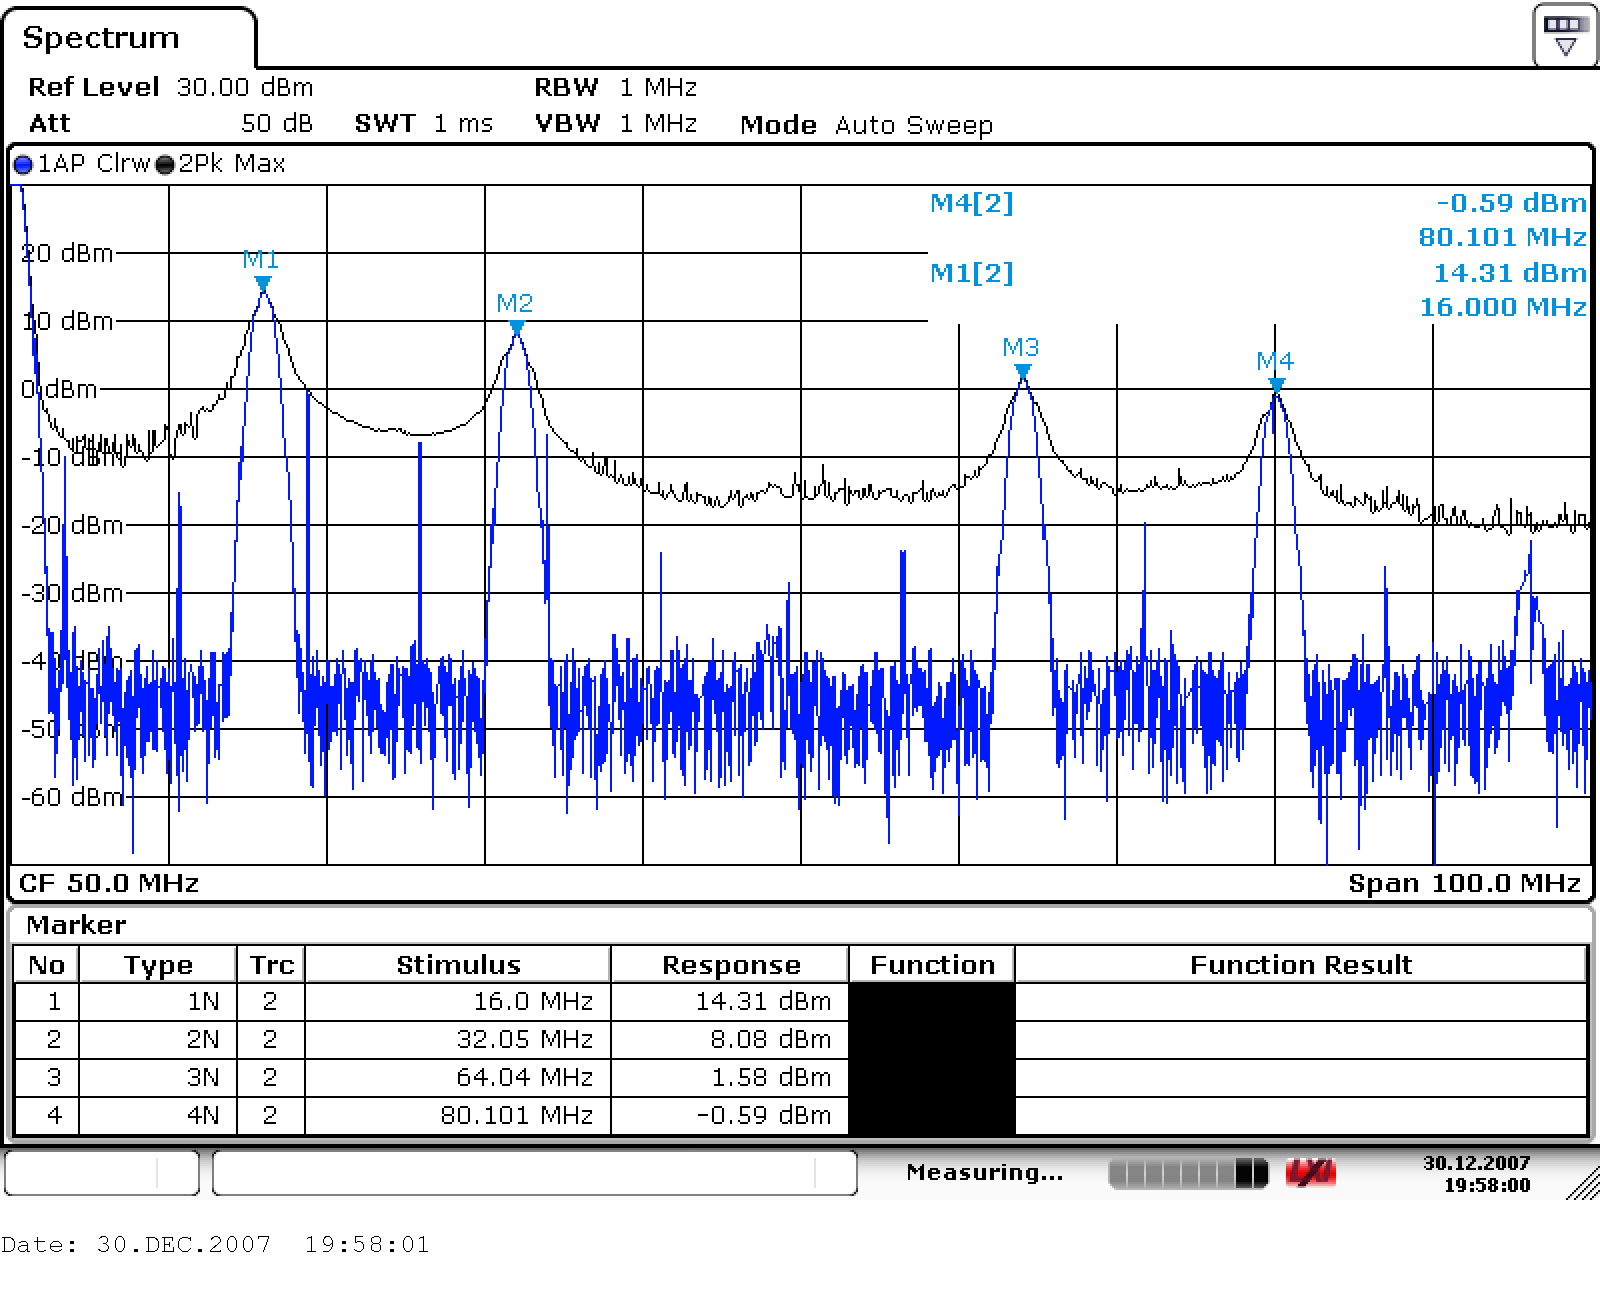
\includegraphics[width=\textwidth,keepaspectratio]{kepek/A_csop_004.PNG}
		\caption{BPSK moduláció}
		\label{fig:modulator_bpsk}
	\end{subfigure}
	\begin{subfigure}[b]{0.49\textwidth}
		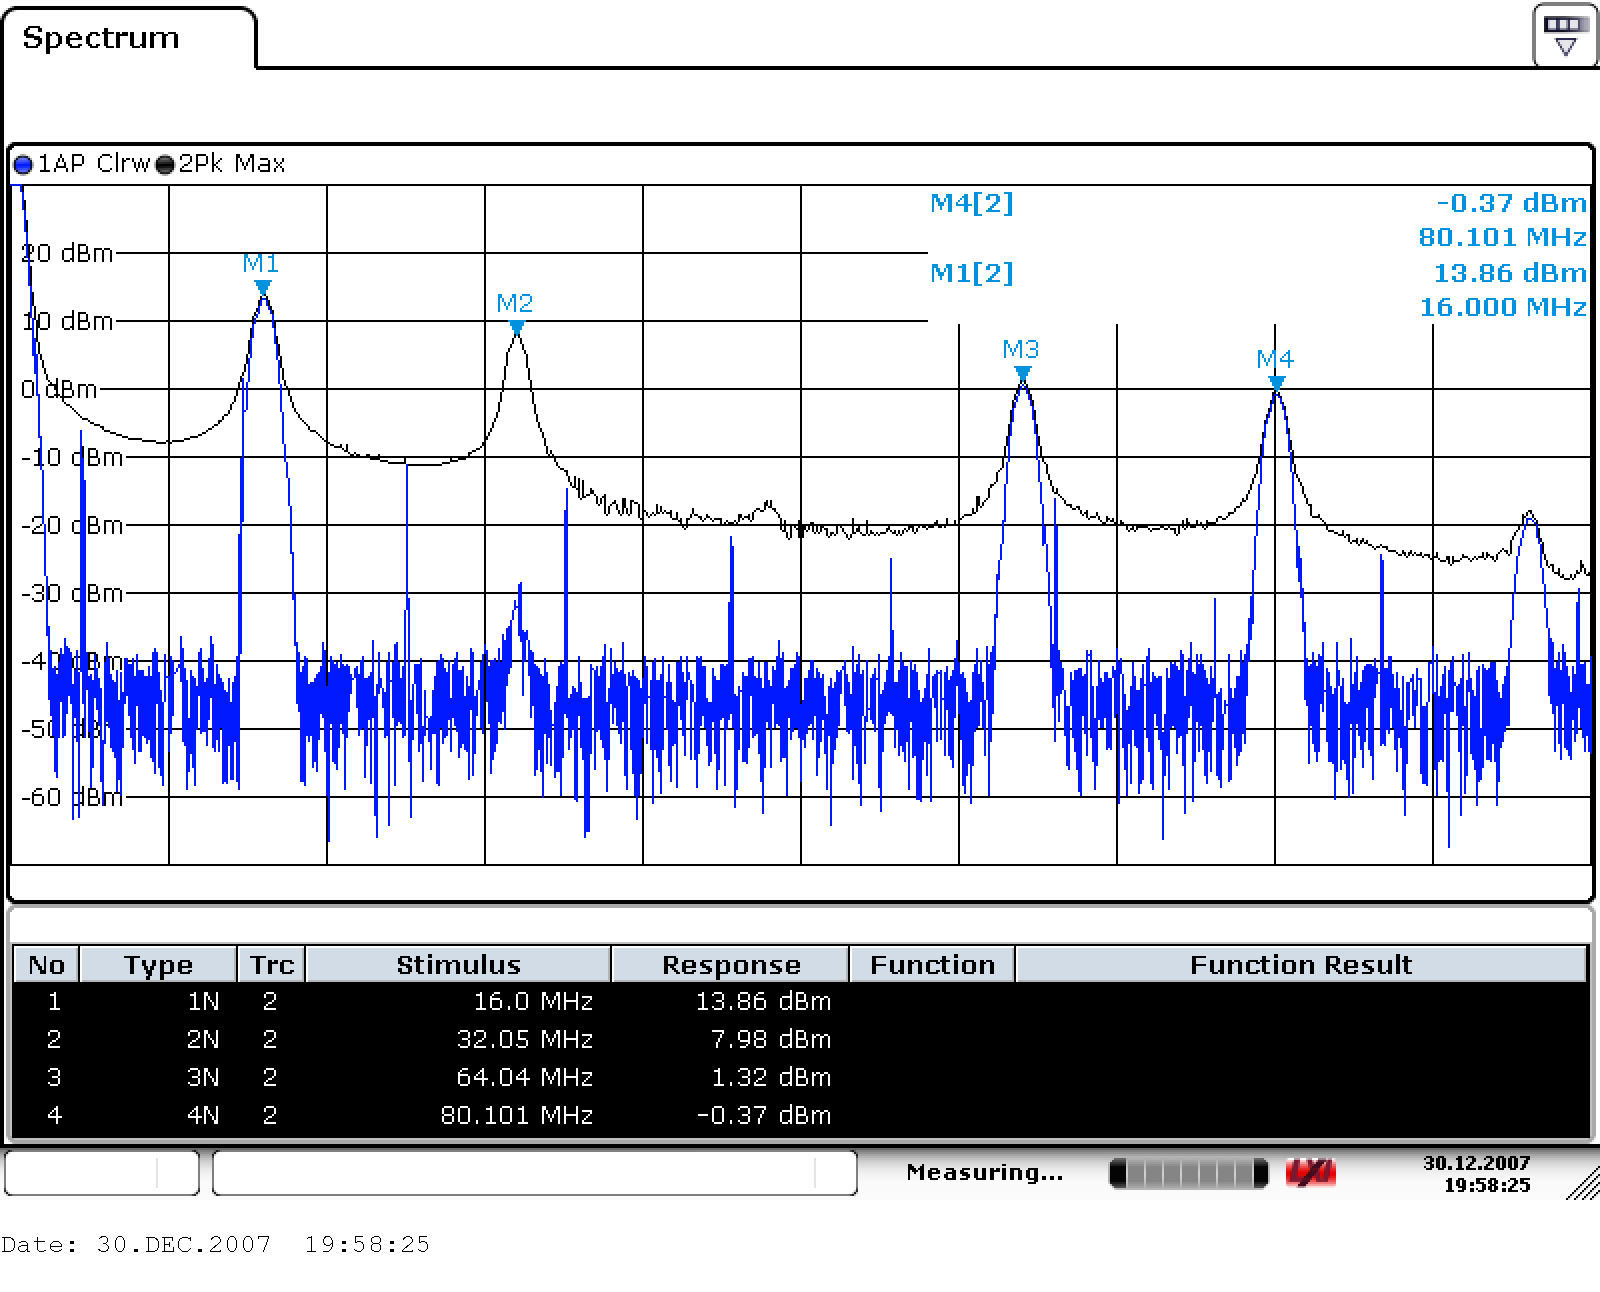
\includegraphics[width=\textwidth,keepaspectratio]{kepek/A_csop_005.PNG}
		\caption{OOK moduláció}
		\label{fig:modulator_ook}
	\end{subfigure}
	\caption{Modulátor szűrés előtti kimenete a két üzemállapotban.}
	\label{fig:modulator}
\end{figure}

Az első, második, negyedik és ötödik harmonikus frekvenciáját és a spektrumanalizátorral mért szintjét az alábbi táblázat foglalja össze mindkét modulációra.
%
\begin{table}[H]
	\centering
	\caption{Harmonikusok frekvenciája és $\si{dBm}$-ben mért szintjei BPSK és OOK moduláció esetén.}
	\label{table:kondi_geometria}
	\begin{tabular}{ | c | c | c |} 
		\hline
		\textbf{Frekvencia}&\textbf{BPSK}&\textbf{OOK}\\
		\hline
		$\SI{16}{MHz}$&$\SI{14.31}{dBm}$&$\SI{13.86}{dBm}$\\
		\hline
		$\SI{32}{MHz}$&$\SI{8.08}{dBm}$&$\SI{7.98}{dBm}$\\
		\hline
		$\SI{64}{MHz}$&$\SI{1.58}{dBm}$&$\SI{1.32}{dBm}$\\
		\hline
		$\SI{80}{MHz}$&$\SI{-0.59}{dBm}$&$\SI{-0.37}{dBm}$\\
		\hline
	\end{tabular}
\end{table}

A jelalakot időben is megfigyelhetjük, ha oszcilloszkópra vezetjük a modulátor kimenetét, ezt mutatja a \ref{fig:modulator_scope}. ábra, a BPSK esetében a fázisváltást látjuk, az OOK-nál bedig a "0/1" átmenetet. A jelalakok láthatóan nem szinuszosak, a felharmonikusok torzítása ellen szűrés szükséges.

\begin{figure}[H]
	\centering
	\begin{subfigure}[b]{0.49\textwidth}
		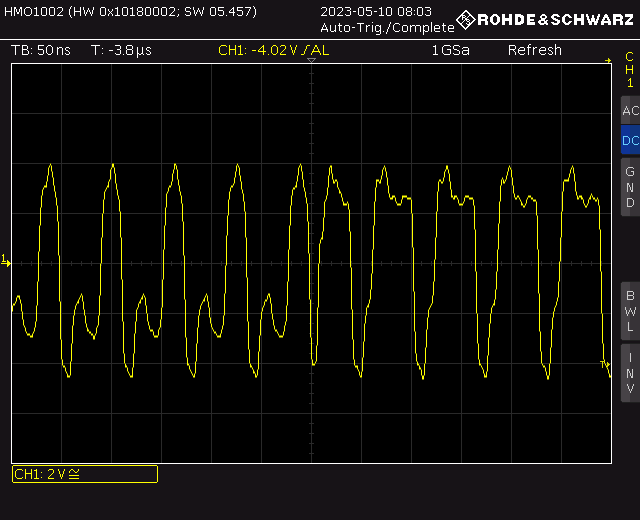
\includegraphics[width=\textwidth,keepaspectratio]{kepek/SCOPE16.PNG}
		\caption{BPSK}
		\label{fig:modulator_bpsk_scope}
	\end{subfigure}
	\begin{subfigure}[b]{0.49\textwidth}
		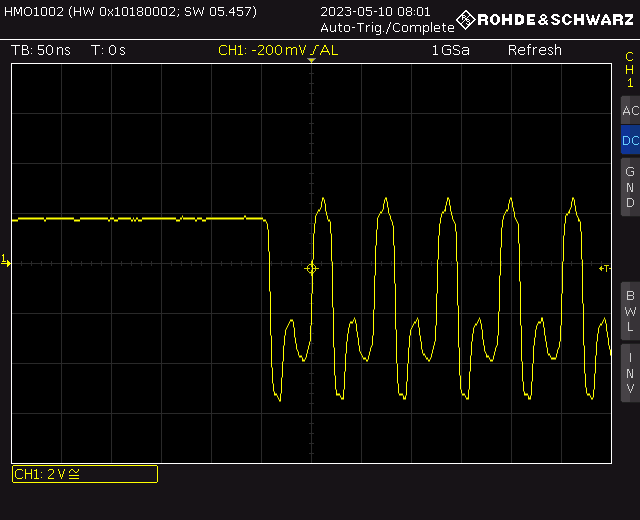
\includegraphics[width=\textwidth,keepaspectratio]{kepek/SCOPE15.PNG}
		\caption{OOK}
		\label{fig:modulator_ook_scope}
	\end{subfigure}
	\caption{Modulátor kimenete oszcilloszkópon.}
	\label{fig:modulator_scope}
\end{figure}

A modulátor kimenetére egy $\SI{16}{MHz}$-es sávszűrőt helyeztünk el, a \ref{fig:modulator_szures}. ábrán bal oldalt a szűretlen maxhold (fekete) és a már szűrt folytonosan mintavételezett jelet (kék) láthatjuk, jobb oldalt pedig már a szűrés utáni maxhold érték szerepel.

\begin{figure}[H]
	\centering
	\begin{subfigure}[b]{0.49\textwidth}
		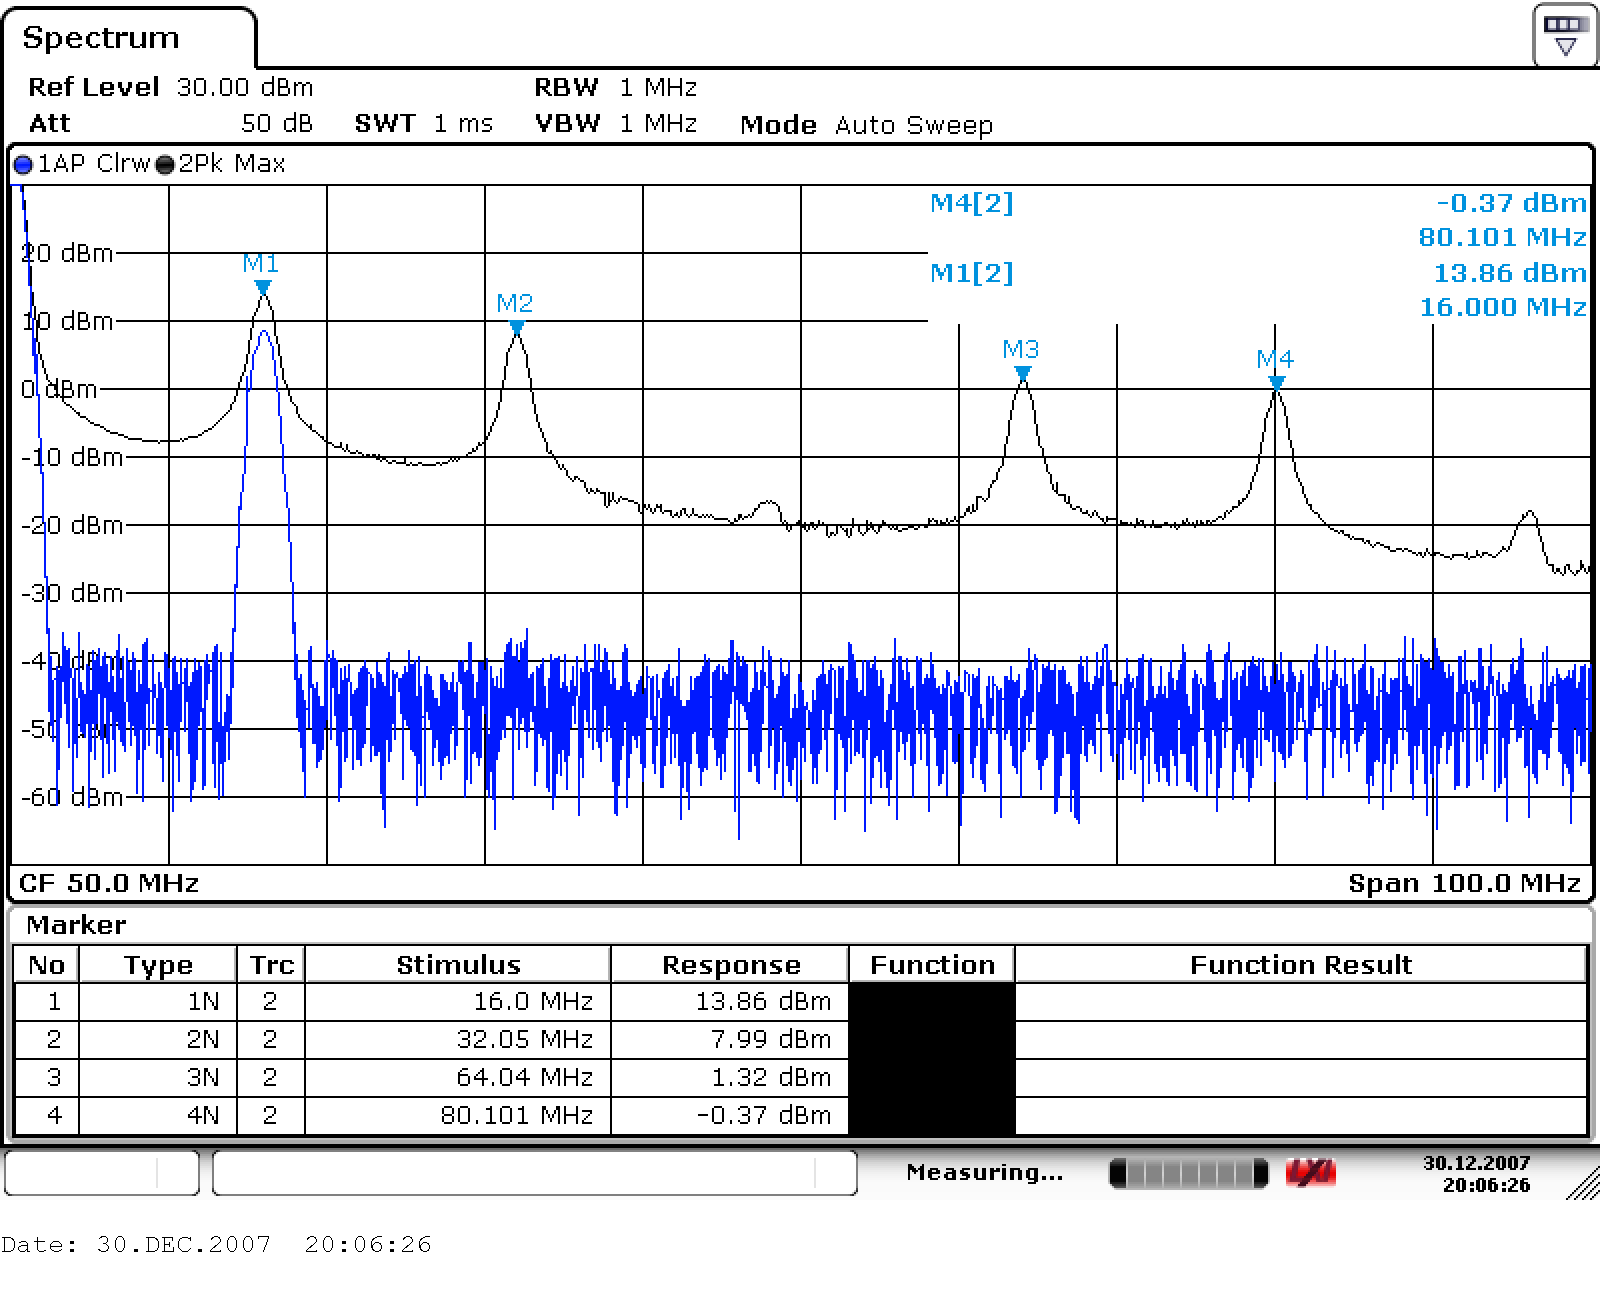
\includegraphics[width=\textwidth,keepaspectratio]{kepek/A_csop_006.PNG}
		\caption{Előtte-utána}
		\label{fig:modulator_szures_elotte}
	\end{subfigure}
	\begin{subfigure}[b]{0.49\textwidth}
		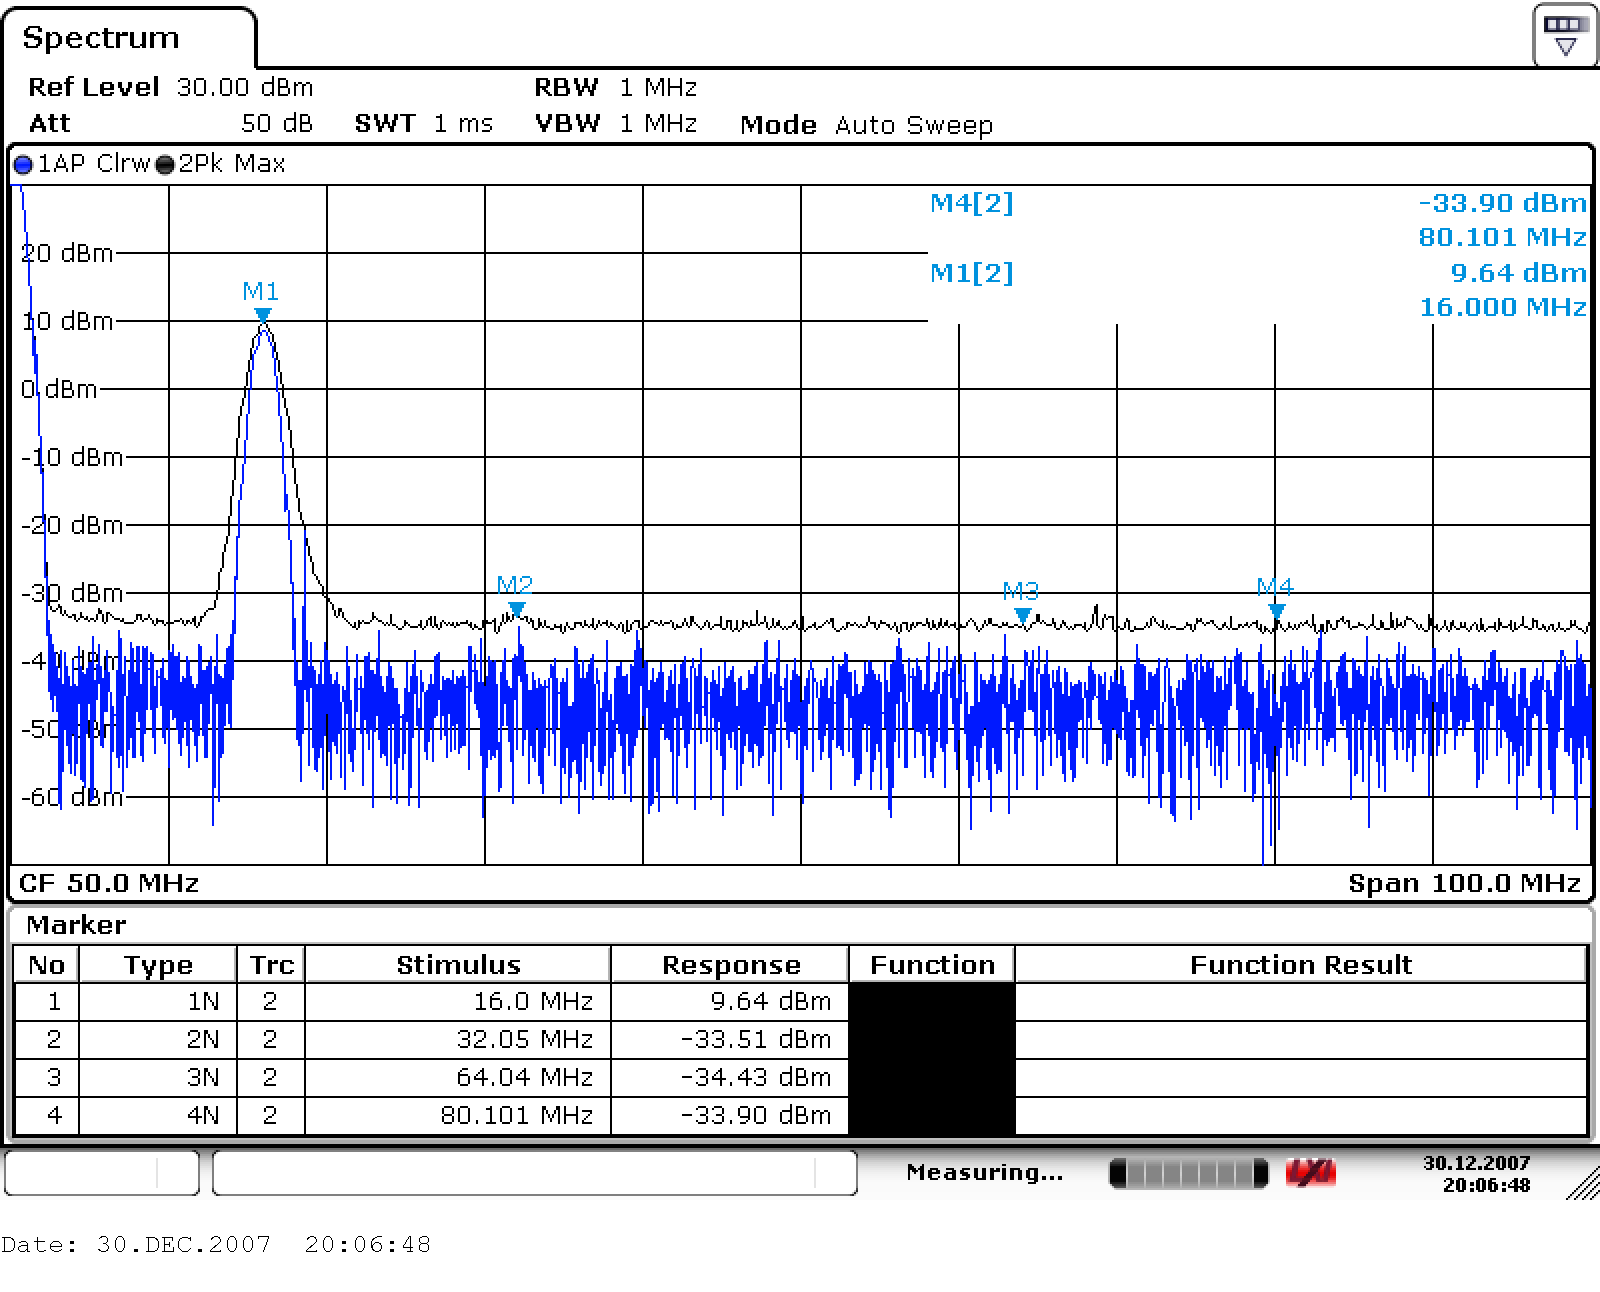
\includegraphics[width=\textwidth,keepaspectratio]{kepek/A_csop_007.PNG}
		\caption{Utána}
		\label{fig:modulator_szures_utana}
	\end{subfigure}
	\caption{Kimeneti spektrum alapsávi szűrés után.}
	\label{fig:modulator_szures}
\end{figure}

A szűretlen esethez hasonlóan megnéztük a két modulációtípust oszcilloszkópon, a \ref{fig:modulator_szures_scope}. ábrán a BPSK-nál a fázisváltás, az OOK-nál az "on/off" átmenet látható. A \ref{fig:modulator_scope}. ábrán látható felharmonikus torzítással ellentétben itt tisztán szinuszos jel mérhető.

\begin{figure}[H]
	\centering
	\begin{subfigure}[b]{0.49\textwidth}
		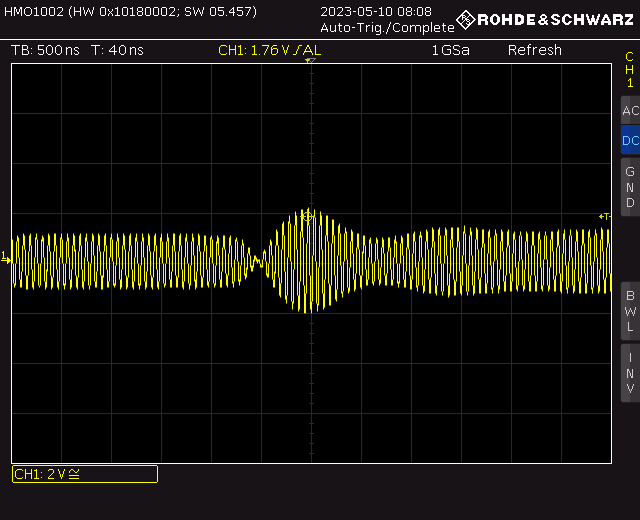
\includegraphics[width=\textwidth,keepaspectratio]{kepek/SCOPE17.PNG}
		\caption{BPSK}
		\label{fig:modulator_bpsk_scope}
	\end{subfigure}
	\begin{subfigure}[b]{0.49\textwidth}
		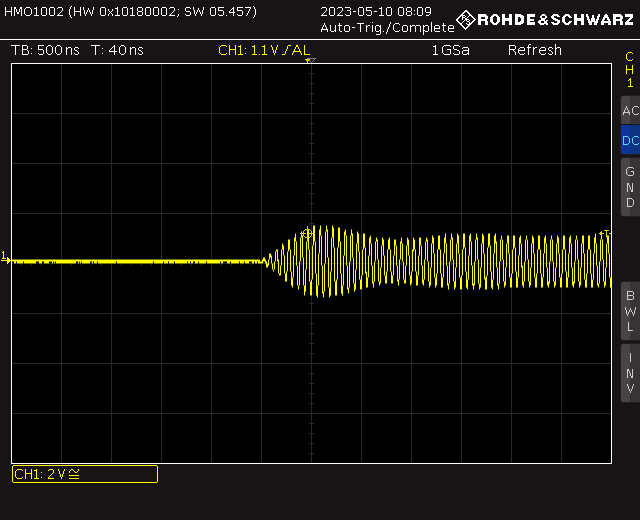
\includegraphics[width=\textwidth,keepaspectratio]{kepek/SCOPE18.PNG}
		\caption{OOK}
		\label{fig:modulator_ook_scope}
	\end{subfigure}
	\caption{Modulátor kimenete szűrés után oszcilloszkópon.}
	\label{fig:modulator_szures_scope}
\end{figure}

Középfrekvenciára, a $\SI{16}{MHz}$-ről $\SI{434}{MHz}$-re való felkeveréshez egy $\SI{450}{MHz}$-es LO-t használtuk, ennek a spektrumát mutatja a \ref{fig:LO_450}. ábra.

\begin{figure}[H]
	\centering
	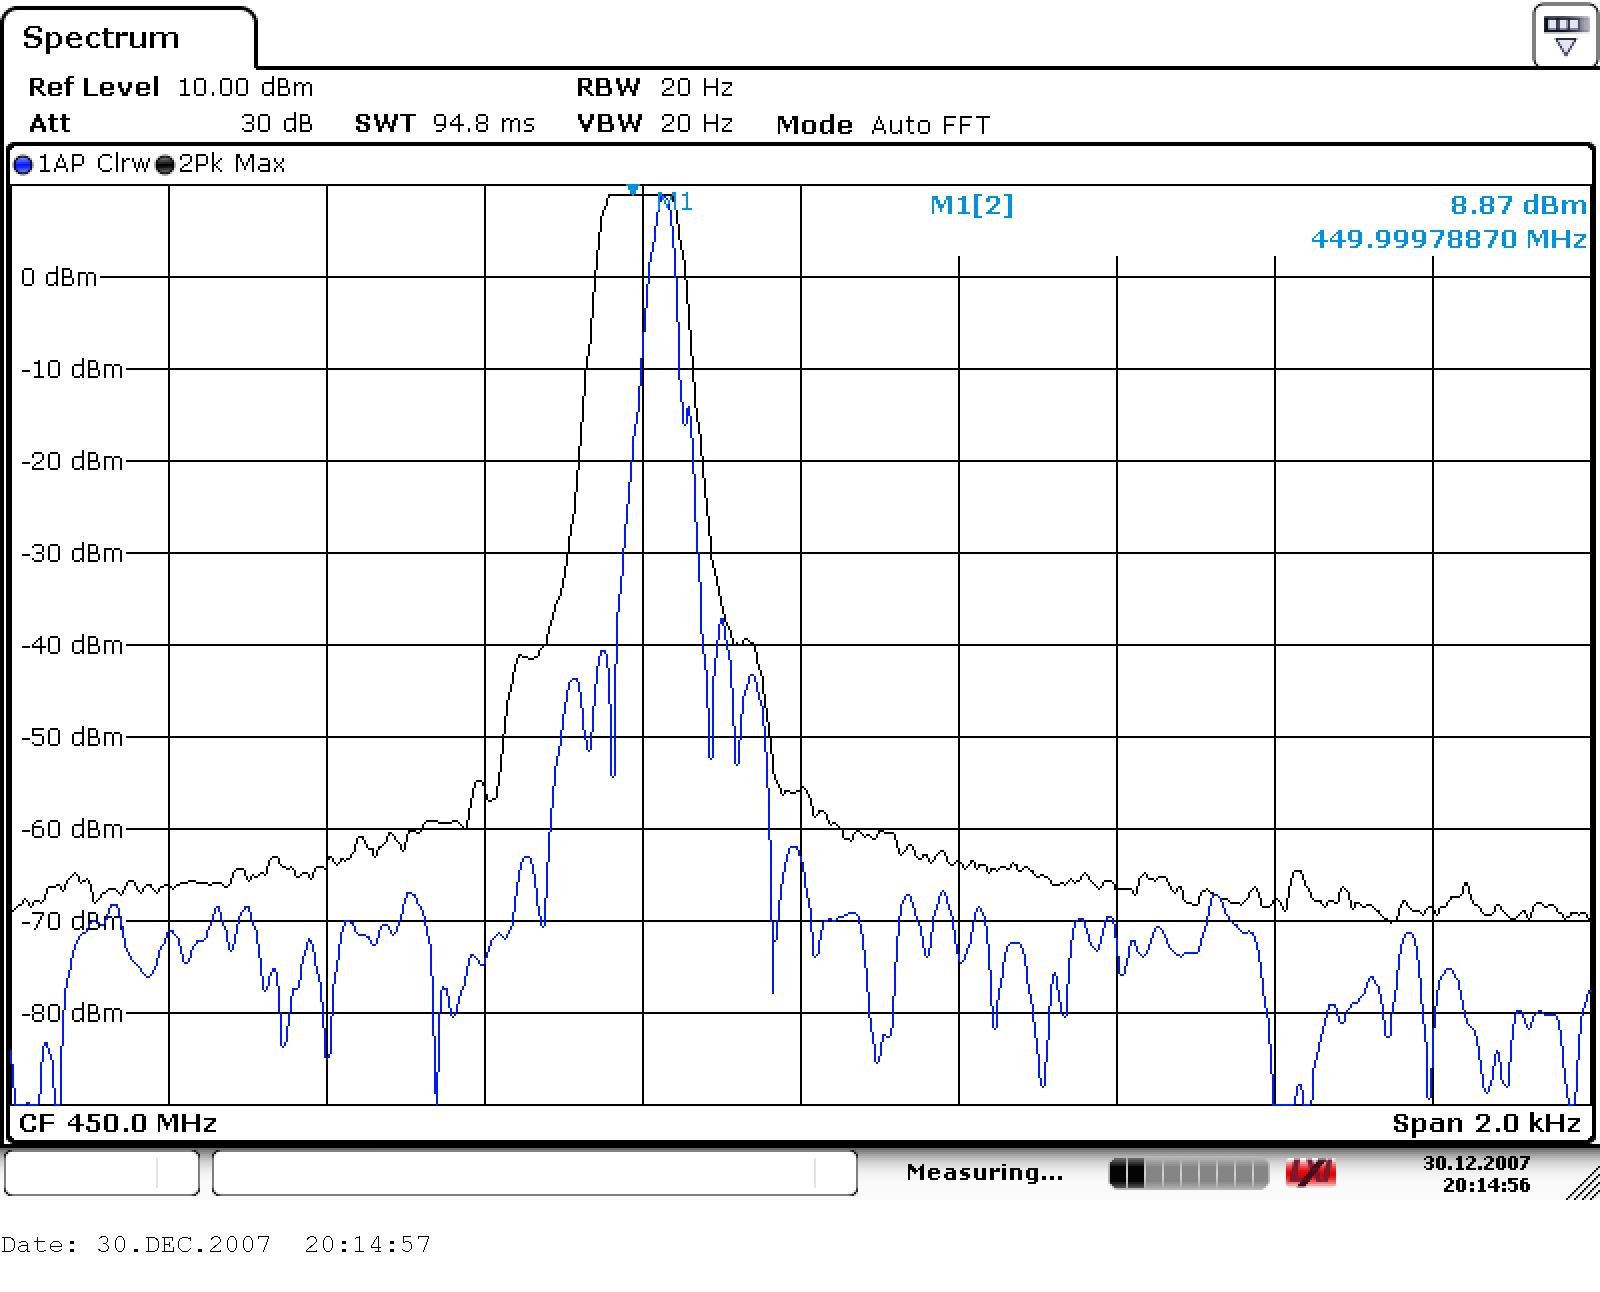
\includegraphics[width=0.5\textwidth,keepaspectratio]{kepek/A_csop_009.PNG}
	\caption{$\SI{450}{MHz}$-es LO spektruma.}
	\label{fig:LO_450}
\end{figure}

Alapszabály, miszerint keverés után szűrni kell, a keveredési termékeket egy $\SI{434}{MHz}$-es sávközepű sávszűrővel nyomjuk el. A szűrés előtti és utáni középfrekvenciás spektrumot a \ref{fig:KF}. ábra mutatja, a hasznos jel közel $\SI{1.7}{dB}$-t, míg a tükörfrekvenciás komponensek $\SI{450}{MHz}$-en és $\SI{466}{MHz}$-en $\SI{40}{dB}$-lel, illetve $\SI{44.5}{dB}$-lel csillapodtak.

\begin{figure}[H]
	\centering
	\begin{subfigure}[b]{0.49\textwidth}
		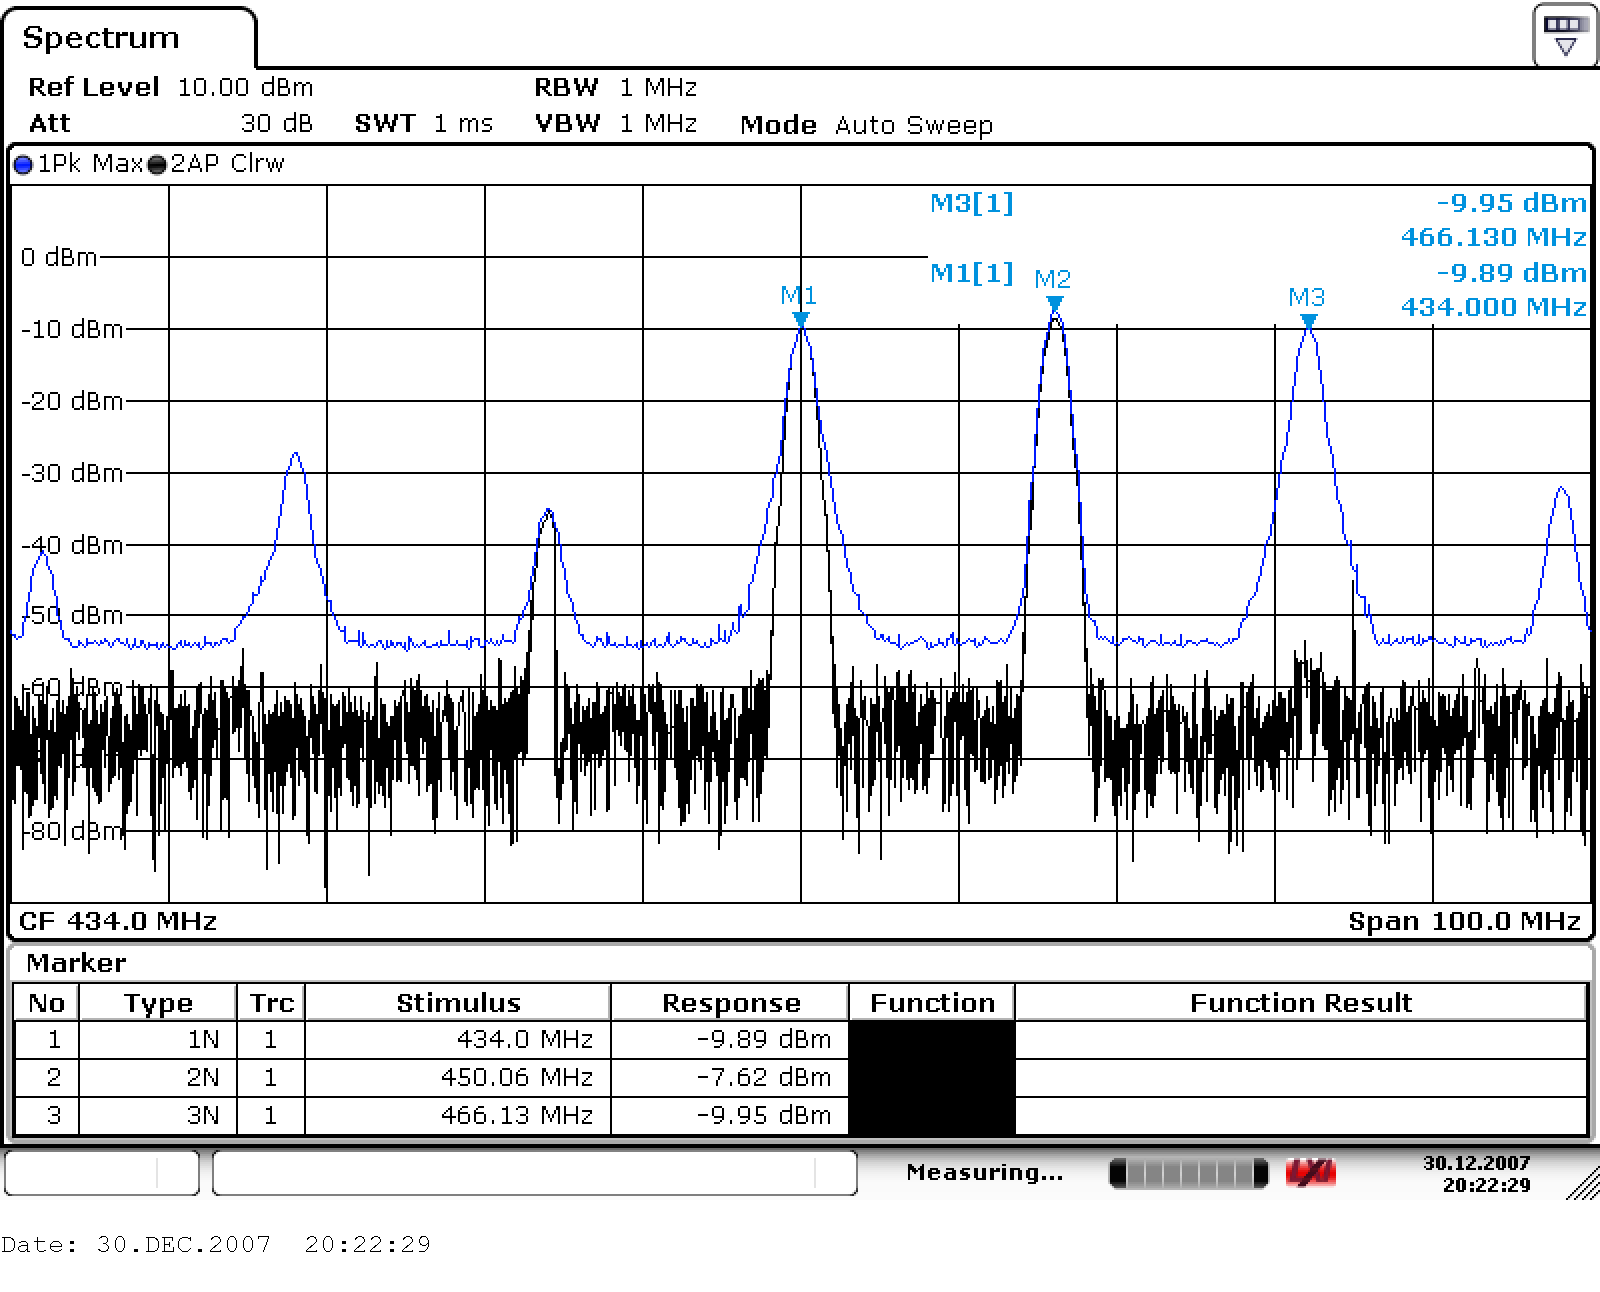
\includegraphics[width=\textwidth,keepaspectratio]{kepek/A_csop_010.PNG}
		\caption{Szűrés előtt}
		\label{fig:KF_elotte}
	\end{subfigure}
	\begin{subfigure}[b]{0.49\textwidth}
		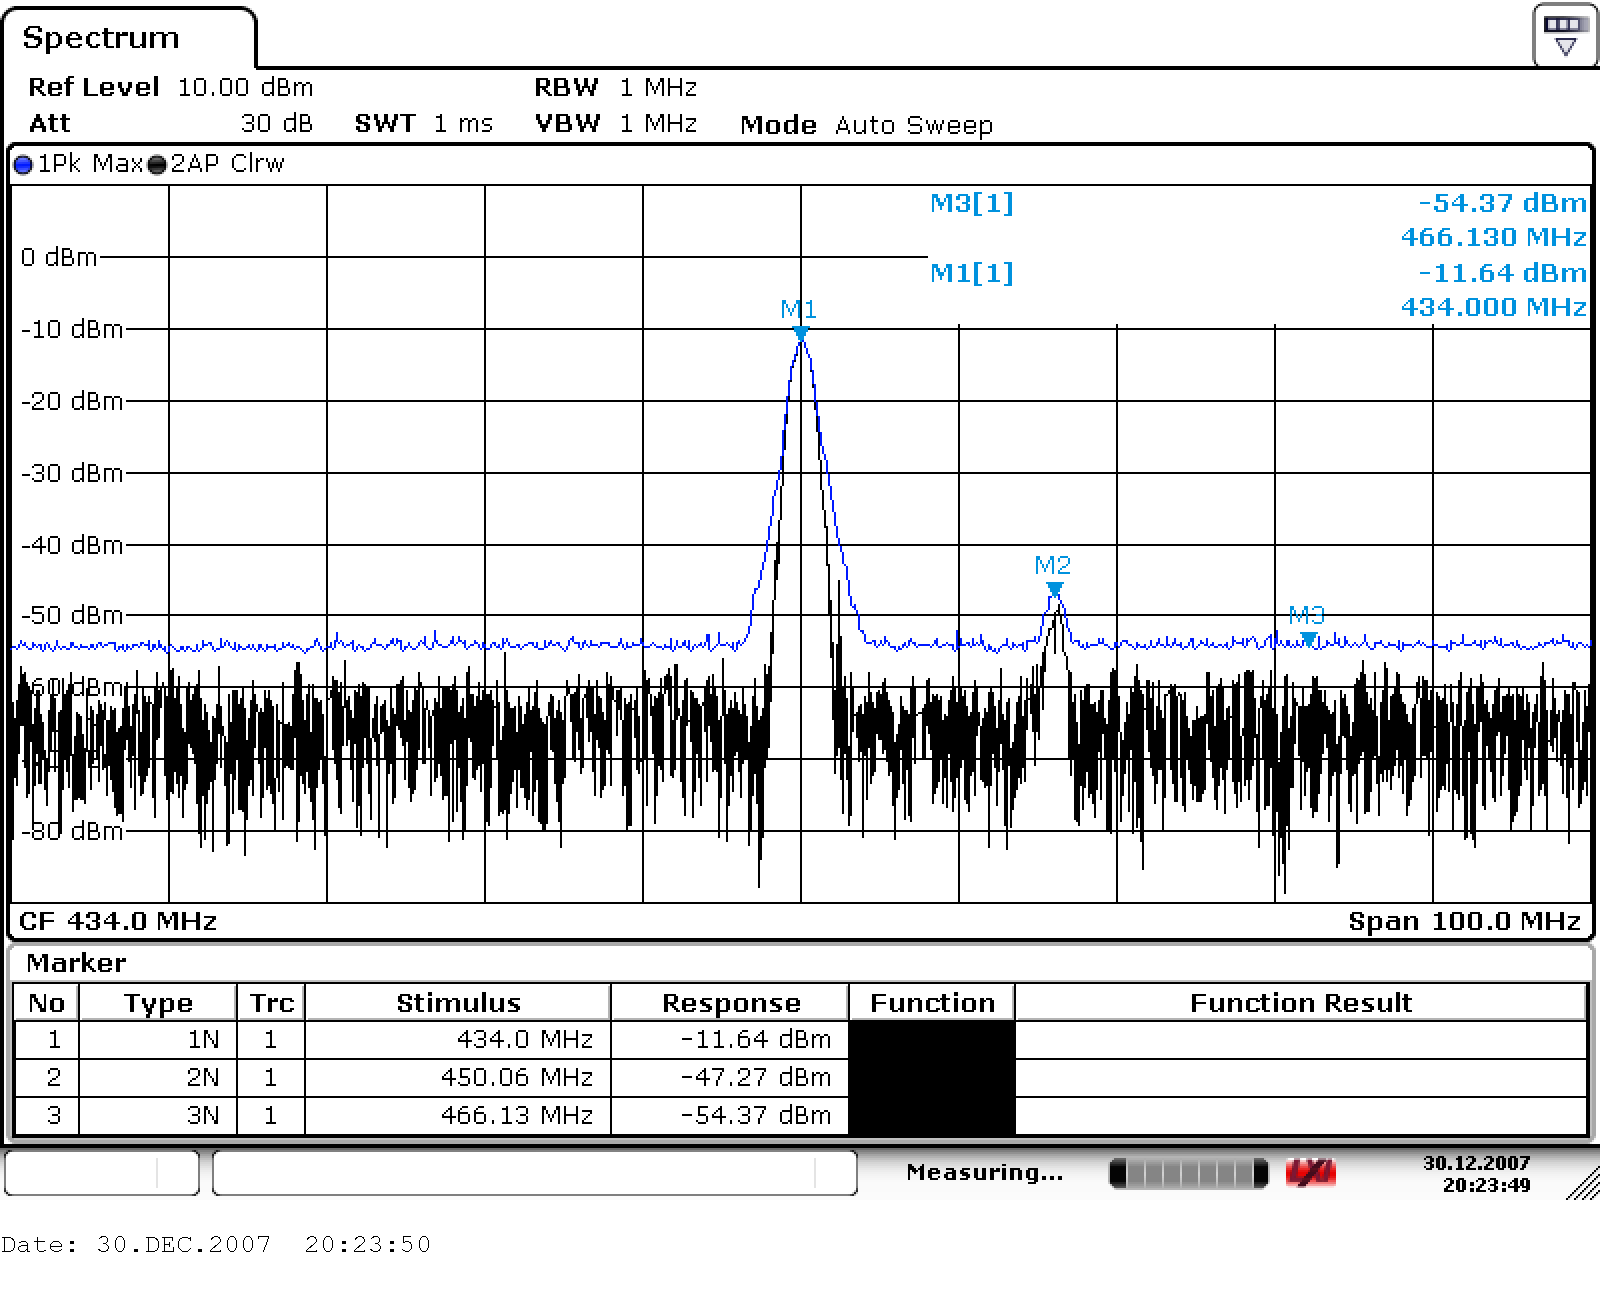
\includegraphics[width=\textwidth,keepaspectratio]{kepek/A_csop_011.PNG}
		\caption{Szűrés után}
		\label{fig:KF_utana}
	\end{subfigure}
	\caption{Középfrekvenciás spektrum szűrés előtt, illetve szűrés után.}
	\label{fig:KF}
\end{figure}

Rádiófrekvenciás fokozatra, a $\SI{434}{MHz}$-ről $\SI{2.4}{GHz}$-re keveréshez egy $\SI{1.966}{GHz}$-es LO szükséges, amit egy fáziszárt hurok, egy PLL áramkör valósít meg. Ennek a spektrumát mutatja a \ref{fig:PLL}. ábra, jobb oldalon kicsi, $\SI{2}{MHz}$-es span mellett vizsgáltuk meg, ahol megfigyelhető a szoknyásodás.

\begin{figure}[H]
	\centering
	\begin{subfigure}[b]{0.49\textwidth}
		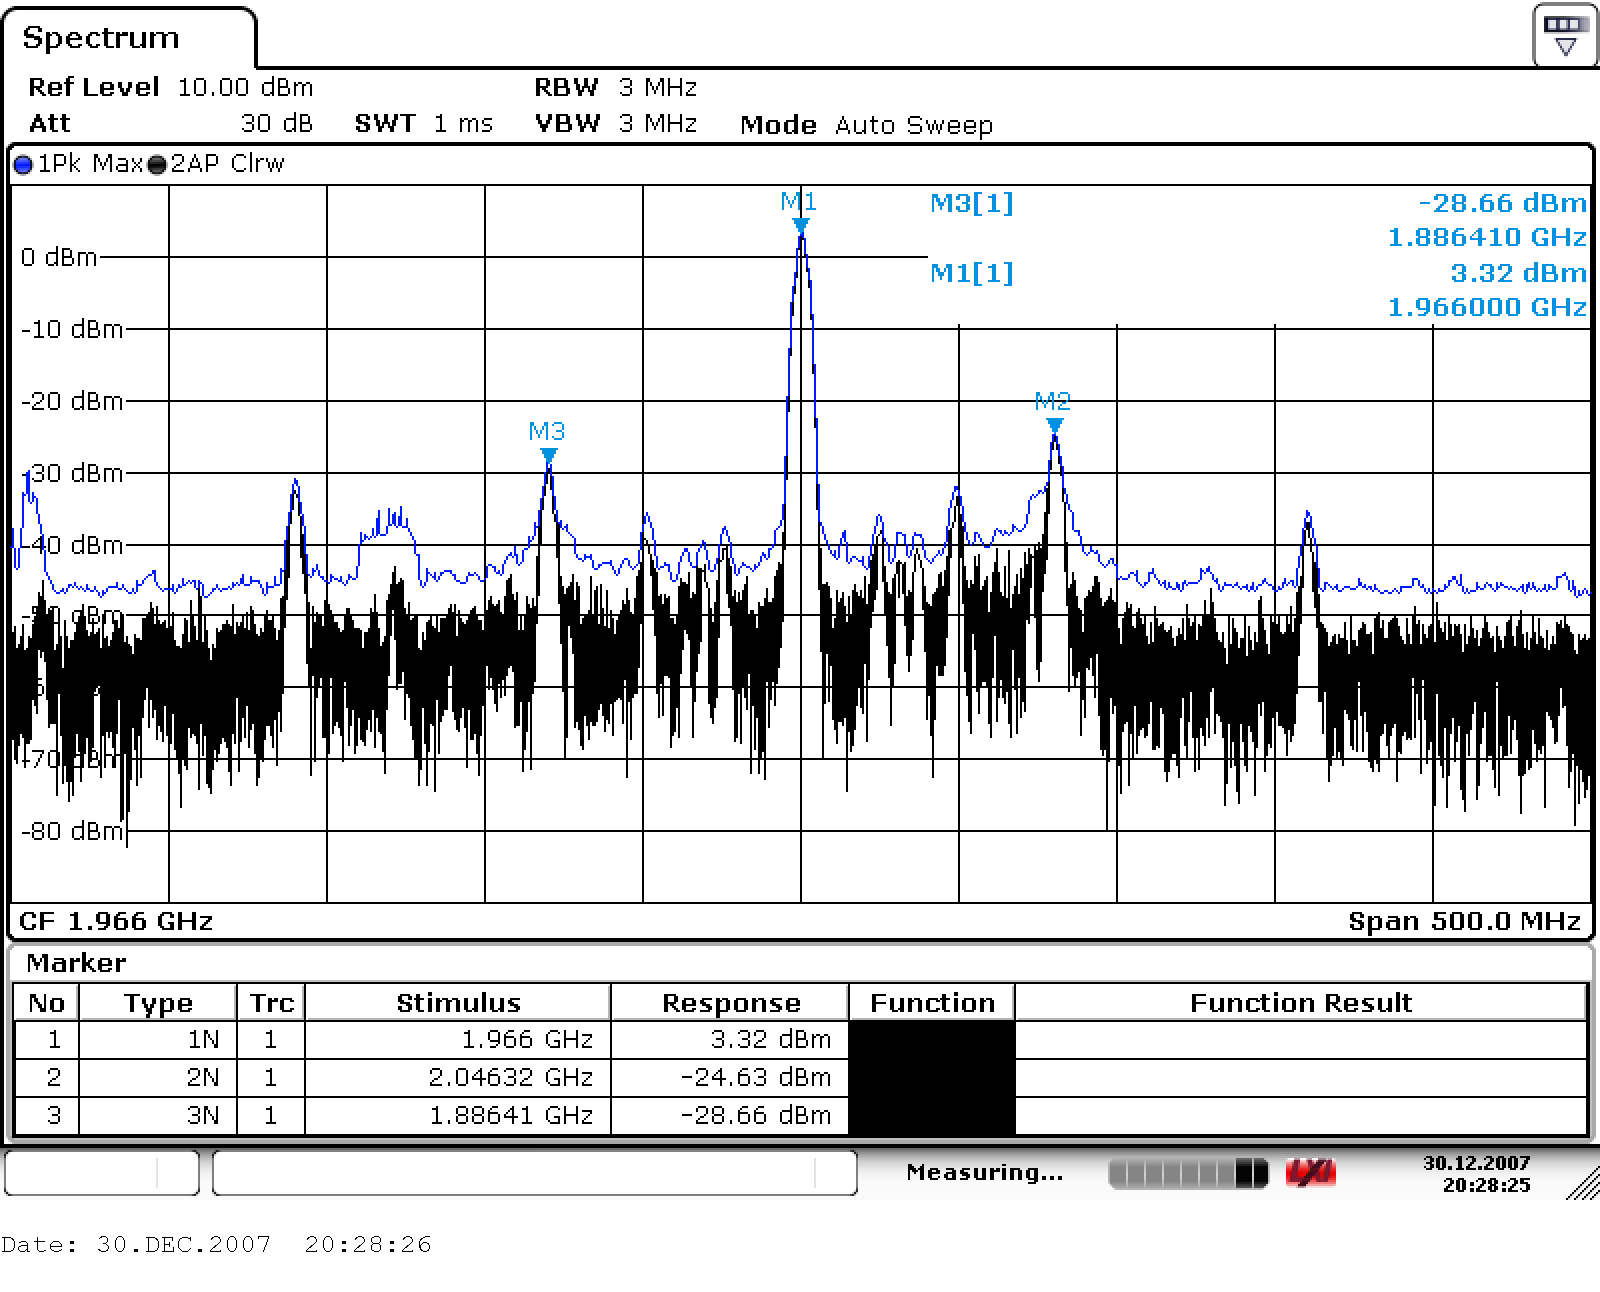
\includegraphics[width=\textwidth,keepaspectratio]{kepek/A_csop_012.PNG}
		\caption{Span = $\SI{500}{MHz}$}
		\label{fig:PLL_span500}
	\end{subfigure}
	\begin{subfigure}[b]{0.49\textwidth}
		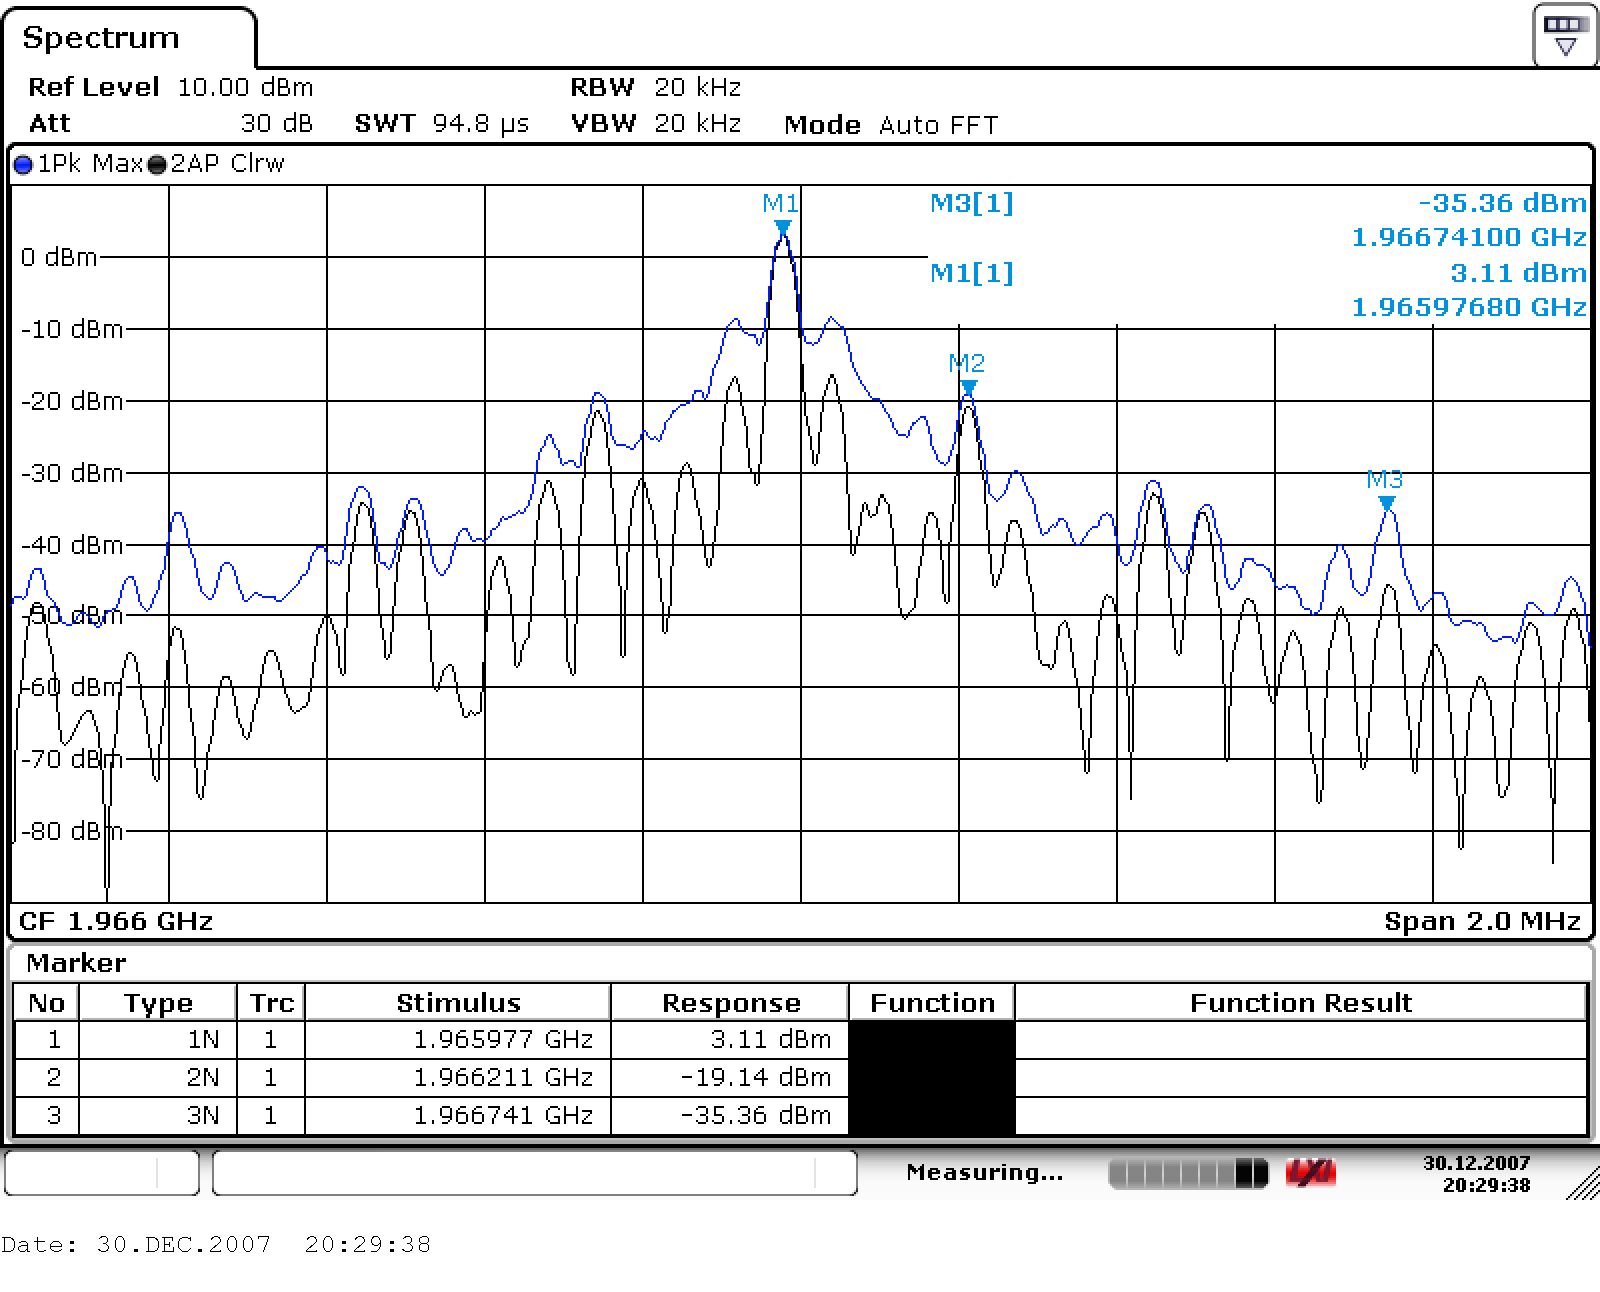
\includegraphics[width=\textwidth,keepaspectratio]{kepek/A_csop_013.PNG}
		\caption{Span = $\SI{2}{MHz}$}
		\label{fig:PLL_span2}
	\end{subfigure}
	\caption{A PLL áramkör kimeneti spketruma.}
	\label{fig:PLL}
\end{figure}

RF keverés után ismét megjelennek keveredési termékek, egy $\SI{2.4}{GHz}$-es sávszűrővel ezek kiszűrhetőek, amint azt a \ref{fig:RF}. ábra mutatja. A hasznos jel $\SI{5.1}{dB}$-lel, a zajkomponensek pedig $\SI{33}{dB}$-lel, illetve $\SI{26.4}{dB}$-lel csillapodtak.

\begin{figure}[H]
	\centering
	\begin{subfigure}[b]{0.49\textwidth}
		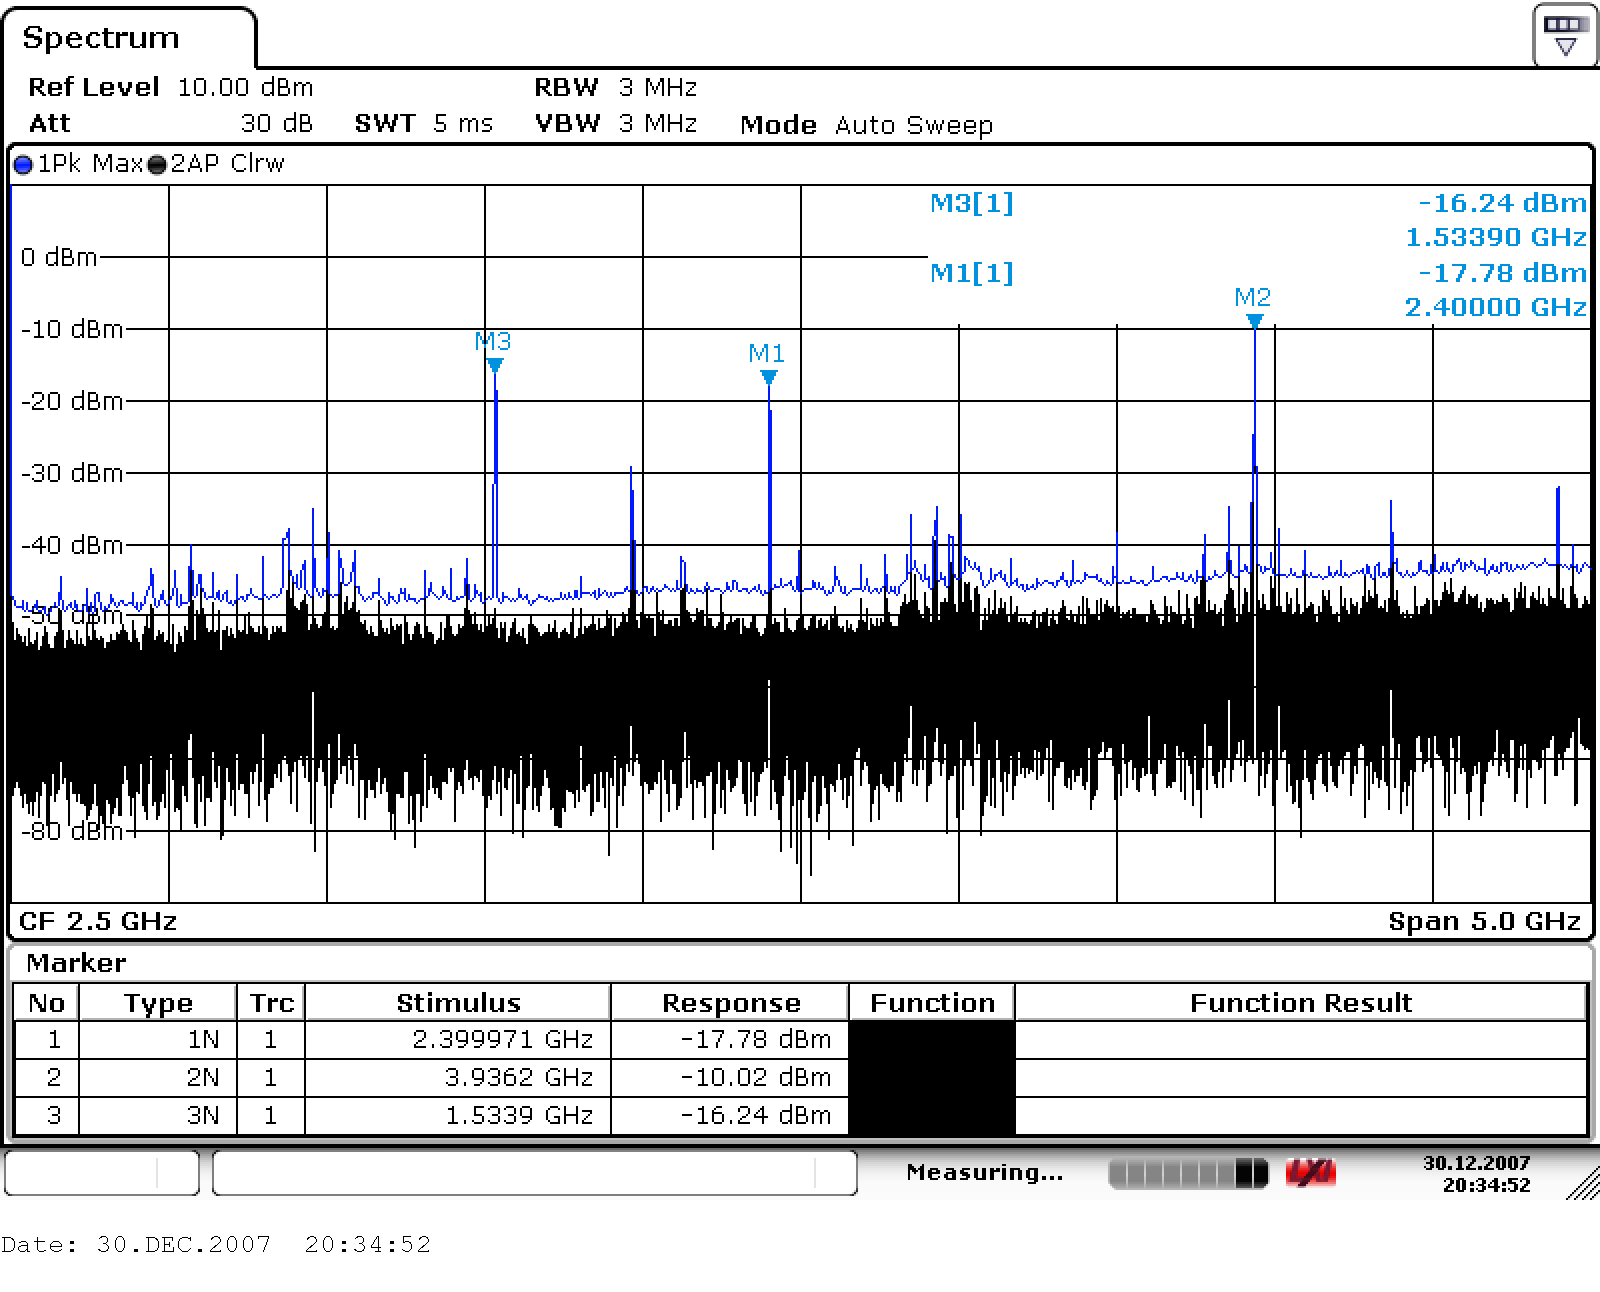
\includegraphics[width=\textwidth,keepaspectratio]{kepek/A_csop_015.PNG}
		\caption{Szűrés előtt}
		\label{fig:RF_elotte}
	\end{subfigure}
	\begin{subfigure}[b]{0.49\textwidth}
		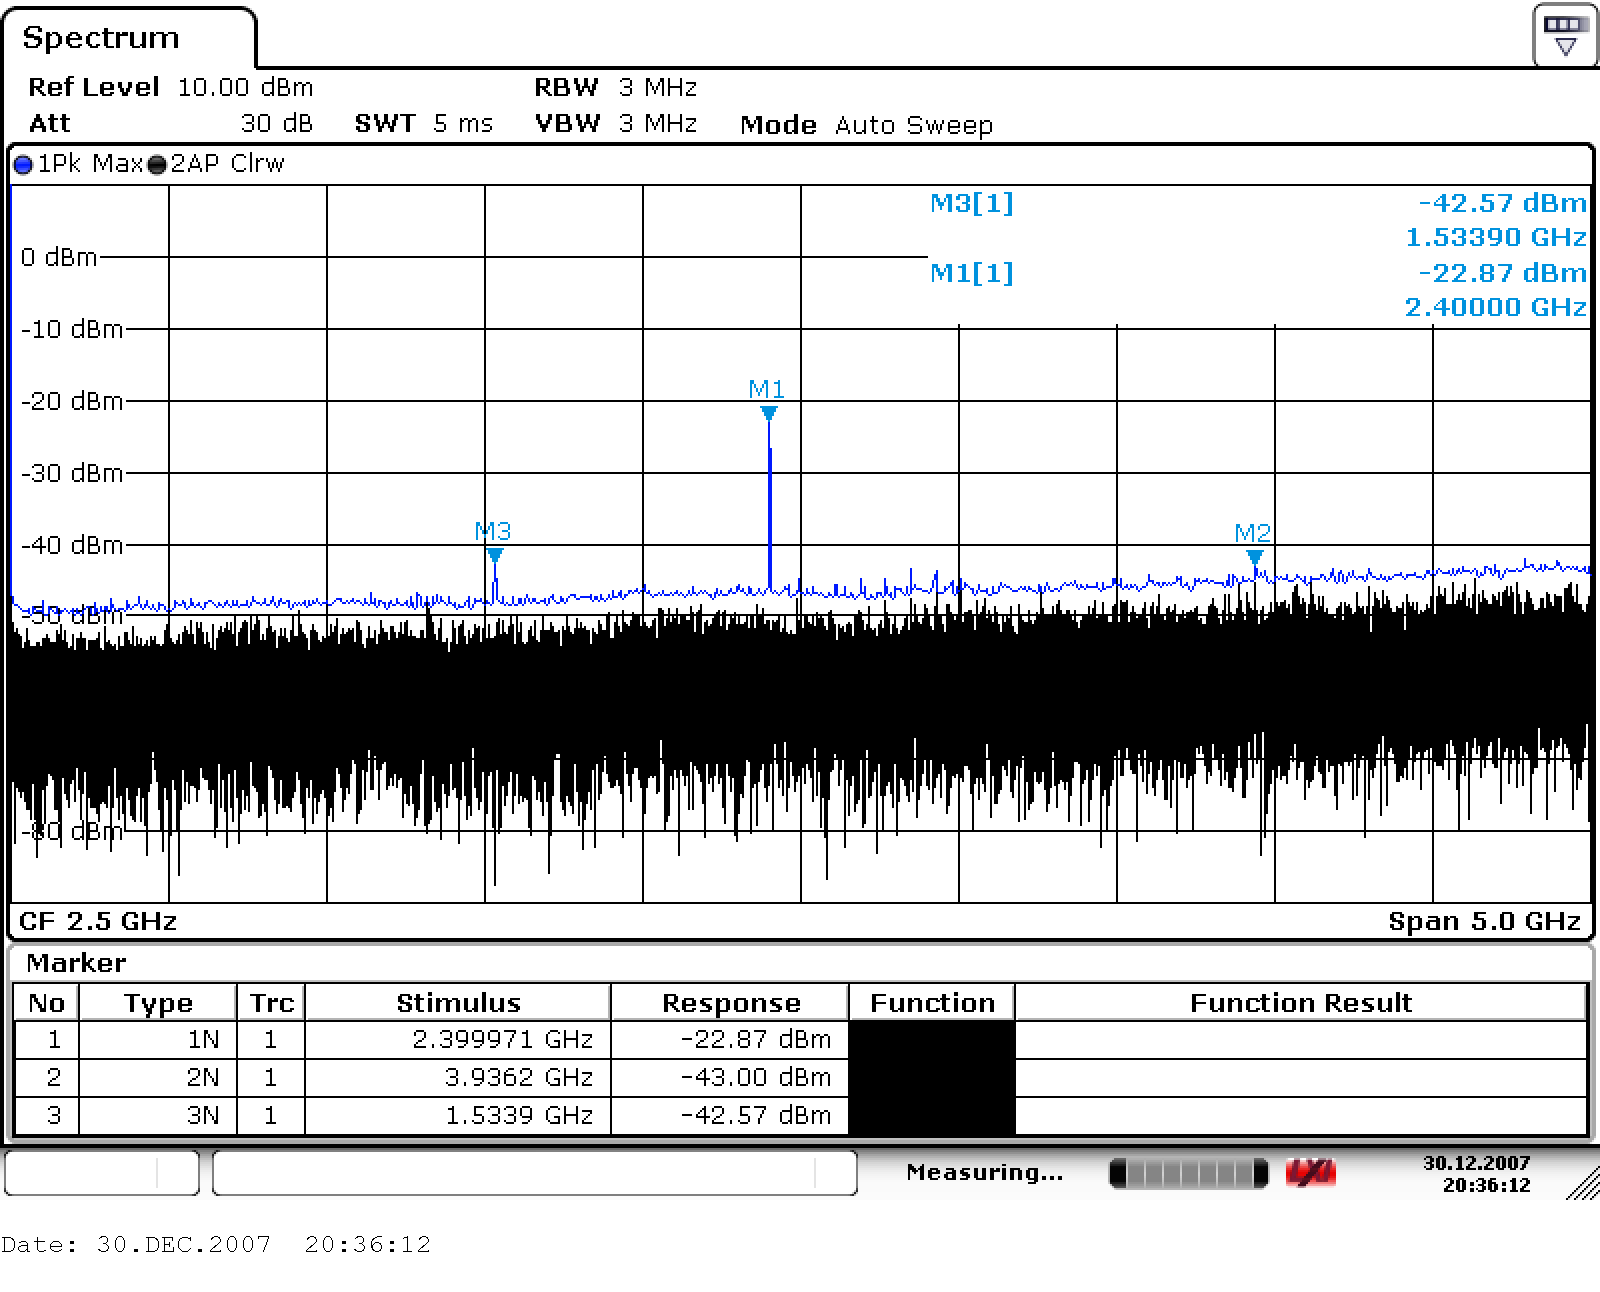
\includegraphics[width=\textwidth,keepaspectratio]{kepek/A_csop_016.PNG}
		\caption{Szűrés után}
		\label{fig:RF_utana}
	\end{subfigure}
	\caption{RF keverés utáni szűrt, illetve szűretlen kimeneti spektrum.}
	\label{fig:RF}
\end{figure}

A teljes összeépített adóláncot, amit a mérés során összeépítettünk a \ref{fig:adolanc}. ábrán láthatjuk.

\begin{figure}[H]
	\centering
	%\includegraphics[width=0.75\textwidth,keepaspectratio]{kepek/?}
	\caption{A teljes adólánc}
	\label{fig:adolanc}
\end{figure}

\section*{Vevőlánc}

% Jancsi, tiéd a pálya




































%\chapter*{Köszönetnyilvánítás}
Ide kerül az opcionális köszönetnyilvánítás, amelyben érdemes megemlíteni a konzulenst, illetve mindazokat, akik a dolgozat létrejöttében segítettek a szerzőnek. 

%\bibliographystyle{IEEEtran}
%\bibliography{tdk.bib}

%\listoffigures
%\listoftables
%\chapter*{Függelék}

A függelék az a fejezet, amely nem képezi szerves részét magának a dolgozatnak (nem növeli az oldalszámot), csak a megértést segíti, illetve a plusz ábrákat, pl. kapcsolási rajzokat, NYÁK terveket, program forráskódokat tartalmazza, de természetesen lehet hivatkozni rá (és sok esetben kell is). \label{fugg}

Jelen dokumentumot, nemcsak pdf, hanem \LaTeX \  forráskód szinten is közzéteszem, abból a megfontolásból, hogy lehetőség szerint legyen egységes a beadott beszámolók és jegyzőkönyvek formátuma és kinézete.

Jelen dokumentum forráskódja példákat tartalmaz a szövegek, képek, táblázatok, számozott és számozatlan felsorolások szerkesztésére, tagolására, formátumára vonatkozóan beleértve a matematika kifejezések forráskód szintű kezelését is.

A LaTeX letölthető többféle operációs rendszerre innen: 
\\
\url{https://www.latex-project.org/get/}

Ha valakinek magyar nyelvű szótárra van szüksége, akkor használhatja jelen dokumentum mappájában levő állományt is: a fordítóban kell beállítani a nyelvi beállításoknál.

\end{document}







